我们需要一种更系统、更严格的方式来描述线程通过内存交互、对共享数据的使用,及其对并发应用的影响,这个描述称为内存模型。内存模型描述了当线程访问相同的内存位置时存在哪些保证和限制。

C++11标准之前,C++语言没有内存模型(在标准中没有提到线程这个词)。这有什么问题呢?再来看看我们的生产者-消费者例子(关注生产者方面):

\begin{lstlisting}[style=styleCXX]
std::mutex mN;
size_t N = 0;
…
new (buffer + N) T( … arguments … );
{ // Critical section start – acquire lock
	std::lock_guard l(mN);
	++N;
} // Critical section end - release lock
\end{lstlisting}

\texttt{lock\_guard}只是一个互斥锁的RAII包装器,所以不能忘记解锁:

\begin{lstlisting}[style=styleCXX]
std::mutex mN;
size_t N = 0;
…
new (buffer + N) T( … arguments … ); // N
mN.lock(); // mN
++N; // N
mN.unlock(); // mN
\end{lstlisting}

请注意,这段代码的每一行都使用了\texttt{N}或\texttt{nM},但从未在一个操作中一起使用。从C++的角度来看,这段代码可化简为:

\begin{lstlisting}[style=styleCXX]
size_t n, m;
++m;
++n;
\end{lstlisting}

这段代码中,操作的顺序并不重要,只要可观察对象的行为没有改变即可(可观察对象的行为是输入和输出,改变内存中的值不是可观察对象的行为),编译器就可以重排它们的顺序。回到最初的例子,为什么编译器不重新对操作进行排序呢?

\begin{lstlisting}[style=styleCXX]
mN.lock(); // mN
mN.unlock(); // mN
++N; // N
\end{lstlisting}

这将是非常糟糕的,但C++标准(直到C++11)无法阻止编译器这样做。

当然,早在2011年之前,我们就已经在用C++编写多线程程序了,那么它们是如何工作的呢?显然,编译器当时没有做这样的优化,原因可以在内存模型中找到。编译器提供了超出C++标准的某些保证,并提供了特定的内存模型,即使标准不需要这些模型。基于Windows的编译器遵循Windows内存模型,而大多数基于Unix和Linux的编译器提供POSIX内存模型和相应的保证。

C++11标准改变了这一点,并赋予了C++内存模型。伴随原子操作的内存序保证,而锁是内存模型的一部分。C++内存模型现在保证了跨平台的可移植性,而以前提供了一组在不同平台上的保证,每个保证都根据其内存模型进行。此外,C++内存模型提供了一些特定于语言的保证。

我们已经在不同的内存序标准中看到了这些保证:自由、获取、释放和获取-释放。C++有一个更严格的内存顺序,称为\textbf{顺序一致}(\texttt{std::memory\_order\_seq\_cst}),这是默认的内存序。不仅每个原子操作都有一个指定顺序的双向内存栅栏,而且整个程序都满足顺序一致性的要求。这个要求表明,程序的行为都按照一个全局顺序执行。此外,这个全局顺序有一个重要的属性。在一个处理器上执行的任意两个操作A和B,使得A在B之前执行。这两个操作必须以全局顺序出现,并且A也在B之前。可以假设一个顺序一致的程序,为每个处理器设想有一组牌,每张牌是具体的操作。然后把这些牌放到一起,而不洗牌。一组牌的牌在另一组牌之间进行移动,但同一组牌的顺序永远不会改变,一组卡片就是程序中操作的全局顺序。顺序一致性是一个理想的属性,因为它使判断并发程序的正确性变得更加容易。然而,这往往会以性能为代价。可以用一个非常简单的基准测试来进行演示,其比较了不同的内存序:

\hspace*{\fill} \\ %插入空行
\noindent
\textbf{05\_barrier\_store.C}
\begin{lstlisting}[style=styleCXX]
void BM_order(benchmark::State& state) {
	for (auto _ : state) {
		x.store(1, memory_order);
		… unroll the loop 32 times for better accuracy …
		x.store(1, memory_order);
		benchmark::ClobberMemory();
	}
	state.SetItemsProcessed(32*state.iterations());
}
\end{lstlisting}

可以使用不同的内存序运行这个基准测试。当然,结果取决于硬件,但下面的结果很罕见:

%\hspace*{\fill} \\ %插入空行
\begin{center}
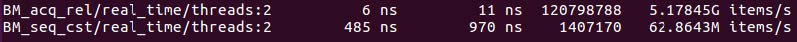
\includegraphics[width=0.9\textwidth]{content/1/chapter5/images/14.jpg}\\
图5.14 -获取-释放与连续一致性内存序的性能
\end{center}

C++内存模型不仅仅是原子操作和内存序。还有,在前面学习伪共享时,假设从多个线程并发地访问数组相邻元素是安全的,这些是不同的变量。然而,语言(甚至编译器)所采用的限制都不能保证。大多数硬件平台上,访问整数数组的相邻元素确实是线程安全的。但对于较小的数据类型(例如\texttt{bool}数组),情况不是这样。许多处理器使用掩码整数写入单个字节,加载包含该字节的整个4字节字,将字节更改为新值,然后将字写回。显然,如果两个处理器同时对共享相同4字节字的两个字节执行此操作,那么第二个写操作将覆盖第一个写操作。C++11的内存模型要求,如果没有两个线程访问同一个变量,那么写入不同的变量(比如数组元素)都是线程安全的。C++11之前,很容易编写一个程序来证明从两个线程写入两个相邻的\texttt{bool}或\texttt{char}变量不是线程安全的。在这本书中没有这个演示的原因是,今天可用的编译器不会退回到C++03,即使指定标准级别为C++03(这是不保证的,编译器可以使用掩码写在C++03模式中写单个字节,大多数编译器使用与C++11模式相同的指令)。

关于C++内存模型的重要性,最后一个例子也有观察的价值,语言和编译器并不都定义了内存模型。硬件有一个内存模型,操作系统和运行时环境有它们的内存模型,程序运行的硬件/软件系统的每个组件都有一个内存模型。整个内存模型,即程序可用的所有保证和限制的集合,是所有这些内存模型的叠加。有时候,可以利用它,例如:在编写特定于处理器的代码时。然而,任何可移植的C++代码都只能依赖于语言本身的内存模型,并且其他底层内存模型都很复杂。

由于语言的内存模型和硬件的内存模型的不同,出现了两种问题。首先,程序中可能有一些在特定硬件上无法检测到的Bug。考虑用于生产者-消费者程序的获取-释放协议。如果犯了一个错误,在生产者端使用释放内存序,而在消费者端使用自由内存序(完全没有栅栏),会期望程序间歇性地产生不正确的结果。但是,如果在x86 CPU上运行这个程序,它似乎是正确的。这是因为x86架构的内存模型是这样的,每个存储都伴随着一个释放栅栏,而每个加载都有一个隐式的获取栅栏。当然,程序仍然存在一个漏洞,如果将其移植到基于ARM的处理器(就像iPad上的处理器)上,它就会给我们带来麻烦。但是在x86硬件上找到这个Bug的唯一方法会用到GCC和Clang中提供的\textbf{Thread santizer(TSAN是一种C/C++数据竞争检测工具)}工具。

第二个问题与第一个问题相反,减少对内存序的限制并不总是会带来更好的性能。在一个x86处理器上从释放到自由内存序写操作不会带来任何性能上的提升,因为总的内存模型可以保证释放顺序(理论上,编译器可能会对自由内存序做更多的优化,而大多数编译器根本不会优化原子操作)。

内存模型为讨论程序如何与内存系统交互提供了科学基础和通用语言,内存栅栏是开发者在代码中用来控制内存模型特性的实际工具。通常,这些栅栏是通过使用隐式调用锁完成的。内存栅栏的最佳使用可以对某些高性能并发程序的效率,产生很大的影响。














